\documentclass[14pt]{extarticle}
\usepackage[T1]{fontenc}
\usepackage[utf8]{inputenc}
\usepackage[russian]{babel}

% page margin
\usepackage[top=2cm, bottom=2cm, left=2cm, right=2cm]{geometry}

% AMS packages
\usepackage{amsmath}
\usepackage{amssymb}
\usepackage{amsfonts}
\usepackage{amsthm}

\usepackage{float}
\usepackage{graphicx}
\usepackage{tabularx}

\usepackage{multirow}

\newcommand{\lb}{\left(}
\newcommand{\rb}{\right)}

\newcommand{\vlevo}{\hspace*{-0.62cm}}

\makeatletter
\setlength{\@fptop}{0pt}
\makeatother

\usepackage{array}
\newcolumntype{C}[1]{>{\centering\let\newline\\\arraybackslash\hspace{0pt}}m{#1}}

\begin{document} 

\begin{titlepage}
\centering
\textbf{\large Московский государственный университет имени М.В.\,Ломоносова\\
\vspace*{0.1cm} Химический факультет\\
\vspace*{0.1cm}
\noindent\makebox[\linewidth]{\rule{\paperwidth}{0.4pt}}
\vspace*{0.1cm}
 Кафедра физической химии}
\vspace*{2cm}

\begin{center}

\includegraphics[width=0.3\textwidth]{pictures/logo.jpg}
\end{center}

\vspace*{2cm}
\Large \textbf{Рентгеноспектральный энергодисперсионный микроанализ} 
\vspace*{6cm}

\begin{flushright}
\large Работа выполнена студентом 515 группы\\
Финенко А.А.\\
\end{flushright}
\vfill
\large\textbf{Москва\\ 2017}
\end{titlepage}

\section*{Теоретический вопрос}
Качественный и количественный РСМА. Его метрологические характеристики. \par

Рентгеноспектральный микроанализ (РСМА) -- это метод определения состава вещества посредством анализа характеристического рентгеновского излучения. Исследуемый объект подвергается воздействию высокоэнергетического электронного пучка, который вызывает рентгеновское излучение. Метод позволяет исследовать микрообъем вещества недеструктивным образом (что верно лишь отчасти; для исследования методом РСМА пригодно весьма ограниченное множество органических объектов, поскольку под действием электронного пучка молекулярная структура может претерпевать изменения). Метод РСМА предназначен для определения элементного состава исследуемого объекта, позволяет проводить как качественный, так и количественный анализ. \par
Задачей качественного анализа является определение всех химических элементов, входящих в состав исследуемого объекта. Качественный анализ применяется, когда о составе объекта неизвестно ничего, и является необходимым шагом перед проведением количественного анализа. Количественный анализ определяет, в каких количественных соотношениях находятся элементы, образующие исследуемый материал. Результатом количественного анализа является процентное содержание каждого химического элемента. (В зависимости от задачи применяют весовые или атомные проценты.) \par
В рамках метода РСМА анализируется состав микрообъема в котором происходит возбуждение рентгеновского излучения электронным пучком (зондом). Размеры этого микрообъема определяются диаметром электронного пучка и свойствами исследуемого вещества. Исследуемый образец должен иметь сток отрицательного заряда с поверхности. В противном случае фокусировка электронного пучка становится невозможной (исследуемая область поверхности накапливает избыточный заряд и начинает отталкивать электронный пучок, что наблюдалось в предыдущих задачах в виде засветки получаемого изображения). Металлические или полупроводниковые образцы закрепляют в проводящем держателе, диэлектрические образцы подвергаются пробоподготовке, заключающейся в напылении тонкой проводящей пленки на поверхность образца ( как правило, углерод, алюминий, серебро, медь или золото). Прежде чем перейти к качественному и количественному анализу методом РСМА, рассмотрим физические основы метода. \par
	Исследуемый образец бомбардируется высокоэнергетическими электронами (обычно 10-15 кэВ), в результате чего с его поверхности происходит эмиссия рентгеновского излучения. Из анализа характеристического рентгеновского излучения определяют, какие элементы и в каких количественных соотношениях присутствуют в образце. 
\subsection*{Генерация рентгеновского излучения}
	Рентгеновское излучение является результатом неупругого взаимодействия между электронами и образцом. Рентгеновское излучение, возникающее при взаимодействии пучка с образцом, бывает двух типов: характеристическое и тормозное. Эмиссия фотонов тормозного излучения происходит, когда электрон испытывает торможение в электрическом поле атома. Электроны, взаимодействуя с отдельными атомами мишени, теряют разное количество энергии. Вследствие этого энергия тормозного излучения имеет непрерывное распределение от нуля до величины ускоряющего напряжения. \par

\begin{figure}[H]
	\centering
	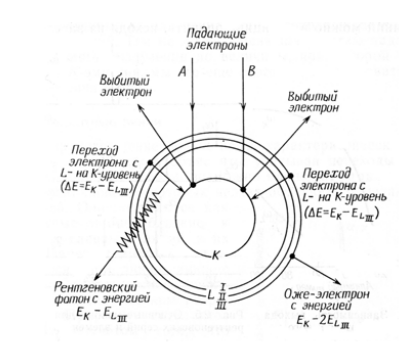
\includegraphics[width = 0.5\linewidth]{./pictures/auger.png}
	\caption{Схема эмиссии характеристического рентгеновского излучения и Оже-электронов под действием электронного пучка}
\end{figure}			
При взаимодействии электрона высокой энергии с атомом, существует вероятность "выбивания"\ одного из электронов внутренней оболочки. Минимальная энергия, необходимая для выбивания с определенного уровня, называется критической энергией ионизации $E_c$. Этот процесс сопровождается переходом атома в ионизированное состояние с вакансией во внутренней оболочке. Переход атома в состояние с меньшей энергией сопровождается переходом одного из электронов внешней оболочки на вакансию. При этом атом излучает квант энергии, величина которого является характеристической. Характеристическая энергия высвобождается из атома двумя способами. Первый способ -- эмиссия рентгеновского фотона с характеристической энергией, специфической для каждого перехода (следовательно, и для определенного элемента). Другим способом является высвобождение электронов Оже. 
В вакансию выбитого электрона могут совершать переход электроны более высоко лежащих оболочек. Каждый такой переход обладает уникальной характеристической энергией. В спектре рентгеновского излучения наблюдается набор характеристических линий. Наиболее интенсивны переходы между соседними глубокими оболочками.
	
\subsection*{Качественный анализ}
Качественный рентгеноспектральный микроанализ возможен благодаря тому, что каждый химический элемент имеет набор характеристических линий на уникальных частотах. Процедура качественного анализа состоит в получении спектра рентгеновского излучения образца и последующей расшифровке. Расшифровка спектра представляет собой идентификацию линий. Возможны ситуации, когда линии различных серий двух элементов накладываются друг на друга. Эта ситуация легко разрешается, поскольку всегда наблюдается целая серия линий для каждого элемента, поэтому идентифицировав остальные линии, можно определить наличествующий элемент в образце. 

\subsection*{Количественный анализ}
Количественный рентгеноспектральный микроанализ -- это относительный метод, основанный на сравнении измеренной интенсивности рентгеновских линий, генерируемых в образце с интенсивностями соответствующих линий в надлежащем стандартном образце известного состава (при заданном токе, ускоряющем напряжении, одинаковой геометрии установки образца и пр.) Содержание элемента рассчитывается из отношения интенсивностей на образце и стандарте с известной концентрацией определяемого элемента. \par
В первом приближении интенсивность излучения характеристической линии $I_A$ (при прочих равных условиях) пропорциональна концентрации элемента. Пусть $c_A$ -- весовая доля элемента A в образце, $c_\textup{эт}$ -- в эталоне. Тогда
\begin{gather}
	\frac{c_A}{c_\textup{эт}} = \frac{I_A}{I_\textup{эт}} \quad \implies \quad c_A = c_\textup{эт} \frac{I_A}{I_\textup{эт}} \notag
\end{gather}

В случае если в качестве эталона выбран чистый элемент
\begin{gather}
		c_A = \frac{I_A}{I_\textup{эт}} = k_A, \quad k_A = \frac{I_A}{I_\textup{эт}} \notag 
\end{gather}

Поскольку эталон и образец представляют разные по составу вещества, то излучение внутри них будет возникать в разных условиях. В связи с этим вводят поправки, учитывающие разницу матриц, в которых находится элемент А (под матрицей здесь подразумевается вещество, в котором находится анализируемый элемент). \par
Разные вещества при одних и тех же характеристиках электронного пучка могут различаться по следующим параметрам: вероятность отражения электрона, средняя глубина проникновения электронов, вероятность возбуждения анализируемого элемента, интенсивность поглощения излучения веществом. Учитывают также возможность вторичной флуоресценции, когда интенсивность излучения одного элемента увеличивается за счет дополнительного возбуждения излучением другого элемента или непрерывным тормозным фоном. Учет всех этих явлений сводят к трем поправкам:
\begin{gather}
		c_A = k_A \cdot Z_A \cdot A_A \cdot F_A, \label{equation}
\end{gather}

\vlevo где 
\begin{itemize}
	\item Z -- поправка на атомный номер
	\item A -- поправка на поглощение
	\item F -- поправка на флуоресценцию
\end{itemize}

\subsection*{Поправка на атомный номер}
Электроны при столкновении с мишенью теряют энергию в результате взаимодействия с атомами мишени. Потери энергии на единицу пути зависят от энергии электронов и среднего атомного номера материала мишени. Поэтому электроны по-разному ведут себя в образце и эталоне. Чем быстрее электроны теряют энергию, тем интенсивнее возбуждают излучение. Для учета этого вводится поправка, называемая тормозным фактором. Кроме того, часть электронов рассеивается обратно и покидает мишень. Доля обратнорассеянных электронов также зависит от среднего атомного номера; чем больше атомный номер, тем больше электронов рассеивается, не потратив энергию на возбуждение излучения. Для учета вышеописанной зависимости вводится фактор, называемый фактором обратного рассеяния. И тормозной фактор, и фактор обратного рассеяния могут сами по себе сильно отличаться для образца и эталона, но из-за тенденции к взаимной компенсации этих двух факторов полная поправка на атомный номер обычно мала (редко превосходит 15\%). Например, в мишени с высоким атомным номером большие потери интенсивности из-за обратного рассеяния электронов в значительной степени компенсируются большей эффективностью, с которой оставшиеся в мишени электроны генерируют рентгеновское излучение. 
\subsection*{Поправка на поглощение}

Поправка на поглощение -- обычно наибольшая из трех поправок, поэтому точность, с которой она рассчитана, существенно влияет на достоверность данных микроанализа. Рентгеновское излучение, прежде чем покинуть образец, проходит в нем некоторое расстояние, которое зависит от глубины генерации фотона. Интенсиновность поглощения излучения веществом зависит от его плотности, а глубина проникновения электронов и генерации излучения зависит от среднего атомного номера вещества. Поэтому условия поглощения в образце и эталоне могут отличаться. \par
Ситуация осложняется также тем, что область генерации рентгеновского излучения имеет заметную протяженность по глубине, условия поглощения на разных глубинах различны.

\subsection*{Поправка на флуоресценцию}
Помимо возбуждения характеристического рентгеновского излучения может возбуждаться вторичное (флуоресцентное) излучение, возникающее в результате ионизации внутренних оболочек атомов при поглощении первичного излучения в образце. Для элемента с атомным номером Z флуоресценция возбуждается только излучением, энергия квантов которого превышает критическую энергию возбуждения $E_c$ соответствующей оболочки элемента. Интенсивность характеристической флуоресценции, а так же излучения, порождаемого непрерывным спектром, зависит от состава образца; вследствие этого необходимо вводить поправку на флуоресценцию, учитывающую различия между образцом и эталоном.

\subsection*{Итеративный метод расчета поправок}
Уравнением \eqref{equation} нельзя воспользоваться непосредственно для определения концентрации $c$ исходя из измеренного соотношения интенсивностей $k$, так как поправки $Z$, $A$ и $F$ сами являются функциями концентрации $c$ (но не $k$). Используют следующую итерационную процедуру. На первом шаге предполагают, что для каждого элемента $c = k$. Оценив таким образом состав вещества, вычисляют поправки $Z$, $A$ и $F$. Подставив полученные поправки в уравнение для каждого элемента, получают более точную оценку их содержания. Затем, используя новые значения содержаний, снова вычисляют поправки. Процесс продолжают до тех пор, пока разница между концентрациями $c_j$ и $c_{j+1}$, полученным в двух последовательных итерациях, станет меньше заданного малого $\varepsilon$. 




\subsection*{Результаты эксперимента}

\begin{figure}[H]
	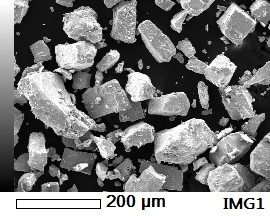
\includegraphics[width = 0.45\linewidth]{./pictures/map1_IMG1.jpg} \hspace{1em}% 
	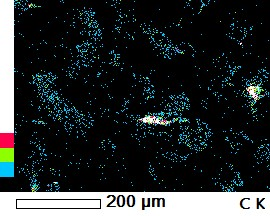
\includegraphics[width = 0.45\linewidth]{./pictures/map1_C_K.jpg} \hspace{1em}%  
	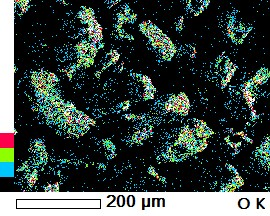
\includegraphics[width = 0.45\linewidth]{./pictures/map1_O_K.jpg} \hspace{1em}% 
	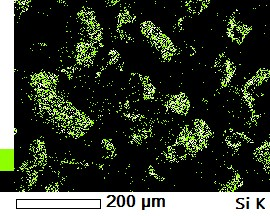
\includegraphics[width = 0.45\linewidth]{./pictures/map1_Si_K.jpg} \hspace{1em}%
	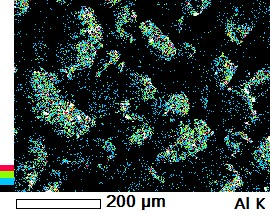
\includegraphics[width = 0.45\linewidth]{./pictures/map1_Al_K.jpg}\hspace{4.2em}%
	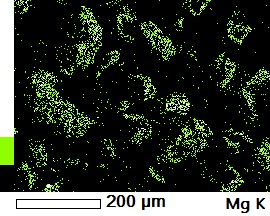
\includegraphics[width = 0.45\linewidth]{./pictures/map1_Mg_K.jpg} \hspace{1em}%
\end{figure}

\begin{figure}[H]
	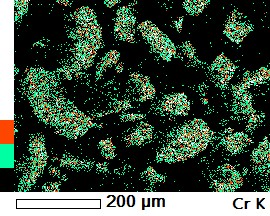
\includegraphics[width = 0.45\linewidth]{./pictures/map1_Cr_K.jpg} \hspace{1em}%
	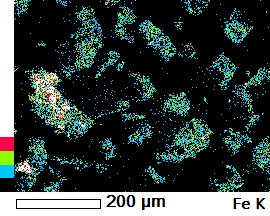
\includegraphics[width = 0.45\linewidth]{./pictures/map1_Fe_K.jpg} \hspace{1em}%
	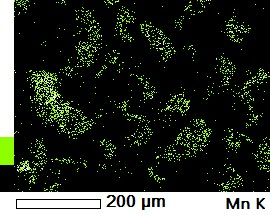
\includegraphics[width = 0.45\linewidth]{./pictures/map1_Mn_K.jpg} \hspace{4.2em}% 
	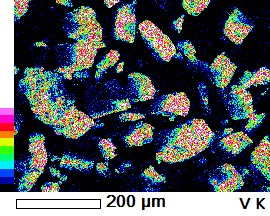
\includegraphics[width = 0.45\linewidth]{./pictures/map1_V_K.jpg} \hspace{1em}%
\end{figure}

Судя по карте распределений элементов, самым распространенным элементов является ванадий. Ванадий равномерно распределен по частицам. Помимо ванадия в частицах присутствуют магний, крмений, алюминий, хром, железо, магний и кислород. В качестве примесного элемента присутствует углерод. 

\begin{figure}[H]
	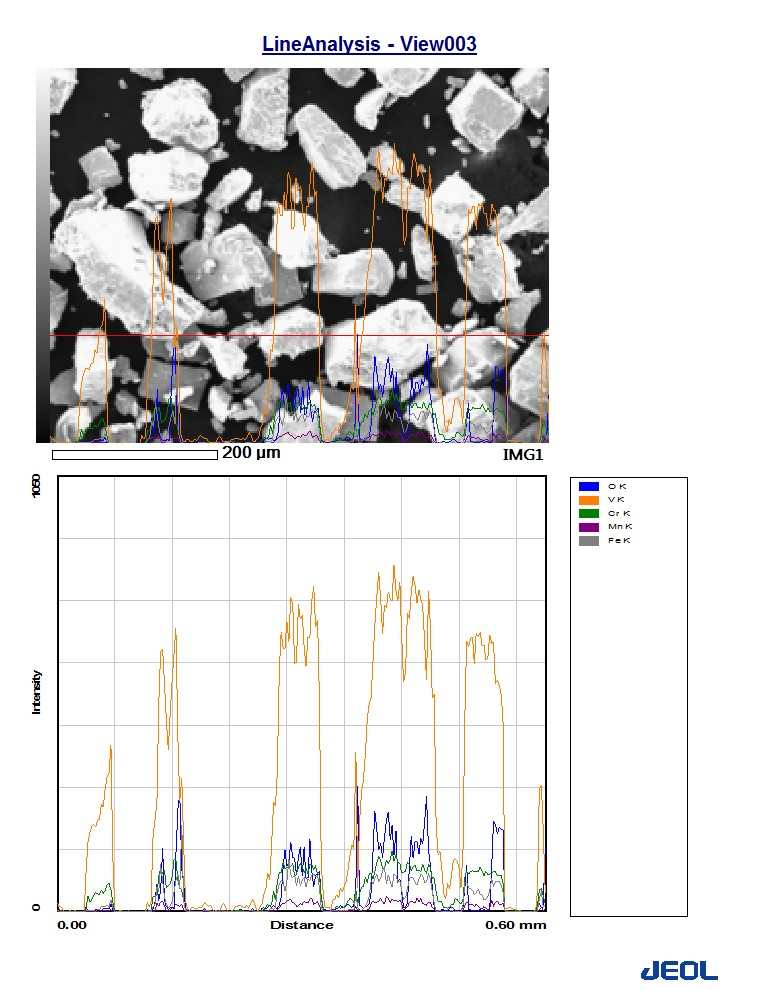
\includegraphics[width = 0.9\linewidth]{./pictures/line_spec_1.jpg}
\end{figure}
\begin{figure}[H]
	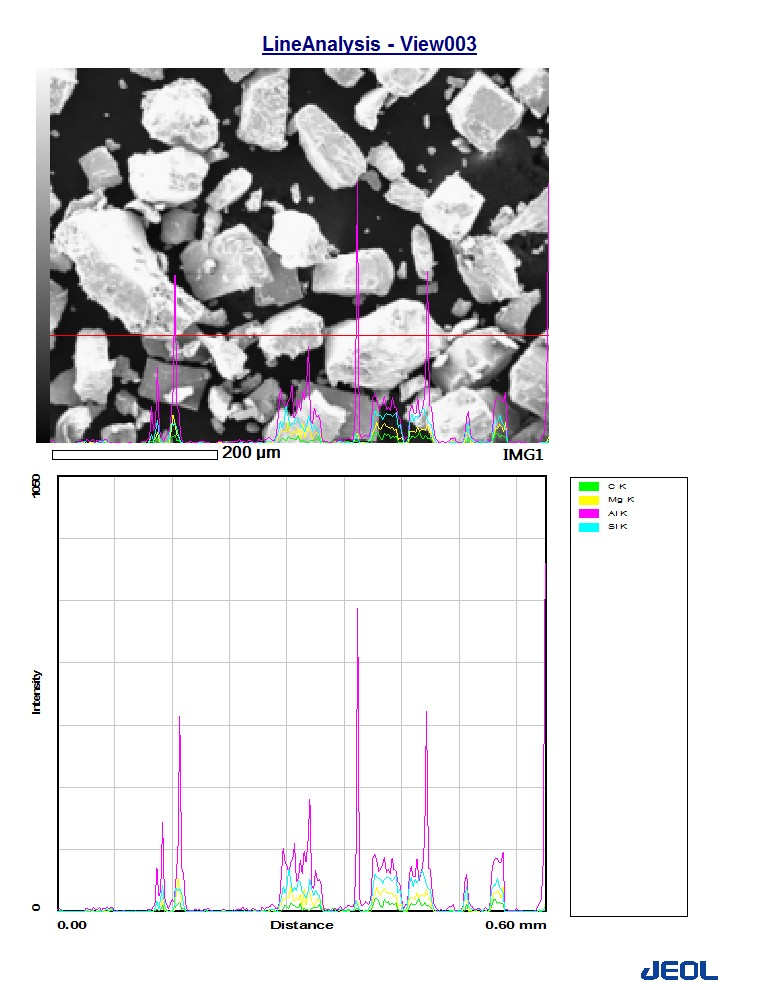
\includegraphics[width = 0.9\linewidth]{./pictures/line_spec_2.jpg}
\end{figure}

Линейное распределение элементов показывает, что основу частиц составляют металлы ванадий, хром, железо и марганец. Сигнал алюминия идет как от частиц, так и от материала подложки.

\begin{figure}[H]
	\includegraphics[width = \linewidth]{./pictures/dot_spec_1.jpg}
\end{figure}

\begin{figure}[H]
	\includegraphics[width = \linewidth]{./pictures/dot_spec_2.jpg}
\end{figure}

\begin{table}[H]
	\centering
	\begin{tabular}{|c|c|c|c|c|c|}
		\hline
		Point & V, \% & Cr, \% & Fe, \% & Mn, \% & Al, \% \\
		\hline
		1 & 75.87 & 0.92 & 13.03 & 1.57 & 2.97 \\
		2 & 71.29 & 0.72 & 12.02 & 1.47 & 3.52 \\
		3 & 68.19 & 0.84 & 11.73 & 1.46 & 3.55 \\
		4 & 90.68 & 2.31 & 3.55 & 0.07 & 1.13 \\
		5 & 78.25 & 1.18 & 12.03 & 1.19 & 3.52 \\
		6 & 75.65 & 0.67 & 12.54 & 1.35 & 3.50 \\
		7 & 76.41 & 4.50 & 3.20 & 0.20 & 5.08 \\
		8 & 82.06 & 2.36 & 1.59 & - & 2.61 \\
		9 & 54.66 & 0.76 & 6.74 & 0.57 & 5.69 \\
		10 & 82.91 & 2.69 & 8.85 & 0.43 & 2.13 \\
		area & 60.42 & 0.99 & 8.15 & 0.75 & 5.054 \\ \hline
		mean & 73.85 & 1.63 & 8.5 & 0.91 & 3.52 \\ \hline
		$\sigma$ & 11.84 & 1.15 & 3.98 & 0.53 & 1.29 \\ \hline
	\end{tabular}
	\caption{Усредненный состав образца по точечным измерения состава} 
\end{table}

\begin{table}[H]
	\centering
	\begin{tabular}{|c|c|c|}
	\hline
	 & $\omega$, \% & $\pm$ d, \% \\
	\hline
		Si & 1.31 & 0.01 \\
		Mn & 1.49 & 0.01 \\
		Cr & 0.185 & 0.005 \\
		C & 0.096 & 0.003 \\
		S & 0.014 & 0.001 \\
		P & 0.022 & 0.001 \\
		Al & 2.12 & 0.03 \\
		Cu & 0.081 & 0.002 \\
		V & 80.1 & 0.1 \\
	\hline
	\end{tabular}
	\caption{Состав феррованадия FeV80}
\end{table}

\subsection*{Список литературы}

\begin{enumerate}
	\item Физические основы рентгеноспектрального микроанализа. Сведенья о методах рентгеноспектрального микроанализа. — СПб.: ЦКП "Материаловедение и диагностика в передовых технологиях"\ при ФТИ им. А.Ф. Иоффе, 2010. — 27 с.
	\item Криштал, М. М. Сканирующая электронная микроскопия и рентгеноспектральный микроанализ в примерах практического применения / М. М. Криштал, И. С. Ясников, В. И. Полунин и др. – М.: Техносфера, 2009. – 208 с.
	\item Количественный электронно-зондовый микроанализ / Под ред. В. Скотта, Г. Лава -- М.: Мир, 1986. -- 352 с.
\end{enumerate}

\end{document}

